\documentclass[parskip=full]{scrartcl}
\usepackage[utf8]{inputenc} % use utf8 file encoding for TeX sources
\usepackage[T1]{fontenc}    % avoid garbled Unicode text in pdf
\usepackage[german]{babel}  % german hyphenation, quotes, etc
\usepackage{hyperref}       % detailed hyperlink/pdf configuration
\hypersetup{                % ‘texdoc hyperref‘ for options
pdftitle={SWT1: Lastenheftvorlage},%
bookmarks=true,%
}
\usepackage{graphicx}       % provides commands for including figures
\usepackage{csquotes}       % provides \enquote{} macro for "quotes"
\usepackage[nonumberlist]{glossaries}     % provides glossary commands
\usepackage{enumitem}

\makenoidxglossaries
%
% % Glossareinträge
%
\newglossaryentry{Dozent}
{
	name=Dozent,
	plural=Dozenten,
	description={Leiter eines oder mehrerer Seminartypen},
}

\newglossaryentry{Kunde}
{
	name=Kunde,
	plural=Kunden,
	description={(Zahlende) Teilnehmer einer oder mehrerer Seminarveranstaltung/en}
}

\newglossaryentry{Seminartyp}
{
	name=Seminartyp,
	plural=Seminartypen,
	description={Typ einer Lehrveranstaltung (z.B. \enquote{Schöner Malen -- Anfängerkurs})}
}

\newglossaryentry{Seminarveranstaltung}
{
	name=Seminarveranstaltung,
	plural=Seminarveranstaltungen,
	description={Tatsächlich stattfindende Lehrveranstaltung (z.B. \enquote{Schöner Malen -- Anfängerkurs, Sommer 2014})}
}

\newglossaryentry{Computer}
{
	name=Computer,
	description={Gerät zur Verarbeitung zur Daten, das die Daten einlesen, verarbeiten, speichern und ausgeben kann}
}

\title{SWT1: Lastenheftvorlage}
\author{Simon Himmel, 2210373}

\begin{document}

\maketitle

%
% % Hinweise - sollen nicht im endgültigen Dokument erscheinen, daher vor der Abgabe löschen!
%
\section{Vorwort}
Die Dokumentation der Pakete ist häufig lesenswert.
Insbesondere bei den Paketen hyperref und scrguide (KOMA-Script).
Wer TeXLivei per Kommandozeile benutzt kann einfach texdoc scrguide aufrufen.
Windows-Benutzer, die noch nie mit Latex gearbeitet haben, können sich alternativ MikTex anschauen; Mac-Benutzer MacTex.

Zum Erzeugen eines PDFs aus den LATEX-Sourcen empfehlen wir einen Wrapper wie latexmk\footnote{\url{https://www.ctan.org/tex-archive/support/latexmk}} oder einen Editor wie TeXStudio\footnote{\url{http://www.texstudio.org/}} zu verwenden.
Dieser übernimmt beispielsweise das mehrfache Ausführen von pdflatex, wo es notwendig ist.

Legen Sie für dieses Dokument ein neues Verzeichnis in Ihrem Git an, zum Beispiel \texttt{image.lastenheft} und speichern Sie alle benötigten Dateien darin.
Speichern Sie keine von Latex generierten Dateien (außer dem PDF) im Git.
Dies geschieht über die mitgelieferte \texttt{.gitignore}.
Sie können aber auch Ihre persönliche \texttt{.gitignore} bei Bedarf erweitern.

\section{Technisches Schreiben}

Technisches Schreiben ist wichtig für alle Arten von technischen und wissenschaftlichen Dokumenten, also auch im PSE und in der Bachelorarbeit.
Es bedeutet vor allem eine präzise Ausdrucksweise und widerspricht dabei einigen Regeln, die man im Deutschunterricht gelernt hat.
Ein paar praktische Tipps (aus den PSE-Dokumenten von Prof. Snelting):
\begin{itemize}[nosep]
\item Vermeide Adjektive.
      Oft (nicht immer) sind sie unnötig oder ein schlechter Ersatz für einen ungenauen Begriff.
\item Nebensatzkonstruktionen vermeiden; Hauptsätze verwenden!
\item Definiere Begriffe klar und verwende keine Synonyme.
      Synonyme lassen offen, ob genau das gleiche gemeint ist oder nur etwas ähnliches.
      Definiere spezielle Begriffe, z.B. \gls{Computer}, in einem Glossar und verweise im Dokument entsprechend darauf.
\item Abkürzungen sollten bei der ersten Verwendung (EV) ausgeschrieben werden.
      Nach der EV reicht dann die Kurzform.
\item Versuche konkrete Zahlen und Namen anzugeben.
      Vermeide ungenaue Ausflüchte wie: meistens, viele, oft, möglichst, üblich, jemand, manche.
\item Viele kurze Sätze sind einfacher zu verstehen als wenige lange Sätze.
\item Beispiele machen das Endprodukt greifbarer.
\item Illustrationen minimalistisch halten (z.B. IKEA Bauanleitung).
      Eine Information, ein Bild.
      Lieber mehrere ähnliche Bilder als ein komplexes Bild.
\item Vermeide Wiederholung, stattdessen Referenzen benutzen.
      Wiederholungen haben oft subtile Unterschiede, was zu Unklarheit und Verwirrung führt.
      Bei Änderungen wird oft vergessen, dass Wiederholungen auch angepasst werden müssen.
\item Versionskontrolle ergibt auch für technische Texte Sinn und nicht nur für Code.
\end{itemize}

%
% % Hier beginnt die Gliederung des Lastenhefts
%
\section{Zielbestimmung}
Die Firma Teachware soll durch das Produkt in die Lage versetzt werden, die von ihr veranstalteten Seminare rechnerunterstützt zu verwalten.

\section{Produkteinsatz}
Das Produkt dient zur Kunden- und Seminarverwaltung der Firma Teachware. Außerdem sollen verschiedene Anfragen beantwortet werden können.

Zielgruppe: die Mitarbeiter der Firma Teachware.

Plattform: PC mit Windows XP oder Nachfolger-Betriebssystem

\section{Funktionale Anforderungen}
\begin{itemize}[nosep]
\item[FA10] Ersterfassung, Änderung und Löschung von \glspl{Kunde} (Teilnehmer, Interessenten).
\item[FA20] Benachrichtigung der Kunden (Anmeldebestätigung, Abmeldebestätigung, Änderungsmitteilungen, Rechnung, Werbung).
\item[FA30] Ersterfassung, Änderung und Löschung von Seminarveranstaltungen und Seminartypen.
\item[FA40] Ersterfassung, Änderung und Löschung von \glspl{Dozent} sowie Zuordnung zu \glspl{Seminarveranstaltung} und \glspl{Seminartyp}.
\item[FA50] Ersterfassung, Änderung und Löschung von Seminarbuchungen.
\item[FA60] Erstellung von Rechnungen.
\item[FA70] Erstellung verschiedener Listen (Teilnehmerliste, Umsatzliste, Teilnehmerbescheinigungen).
\item[FA80] Anfragen der folgenden Art sollen möglich sein:
     Wann findet das nächste Seminar X statt? Welche Mitarbeiter der Firma Y haben das Seminar X besucht?
\end{itemize}

\section{Produktdaten}
\begin{itemize}[nosep]
\item[PD10] Es sind relevante Daten über die Kunden zu speichern.
\item[PD20] Falls ein Kunde zu einer Firma gehört, dann sind relevante Daten über die Firma zu speichern.
\item[PD30] Es sind relevante Daten über Seminarveranstaltungen, Seminartypen und Dozenten zu speichern.
\item[PD40] Bucht ein Kunde eine Seminarveranstaltung, dann sind entsprechende Buchungsdaten zu speichern.
\end{itemize}

\section{Nichtfunktionale Anforderungen}
\begin{itemize}[nosep]
\item[NF10] Die Funktion /FA80/ darf nicht länger als 15 Sekunden Interaktionszeit benötigen, alle anderen Reaktionszeiten müssen unter 2 Sekunden liegen.
\item[NF20] Es müssen maximal 50.000 Teilnehmer und maximal 10.000 Seminare verwaltet werden können.
\end{itemize}

\section{Systemmodelle}

\subsection{Szenarien}

\subsection{Anwendungsfälle}
\subsubsection{Seminarorganisation}
\begin{center}
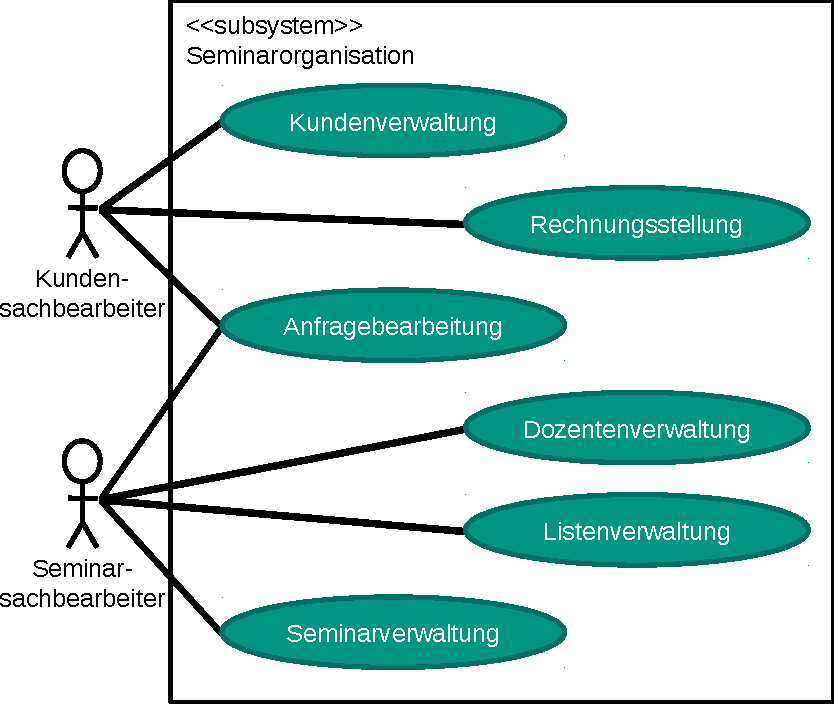
\includegraphics[width=0.8\textwidth]{szenario_seminarorganisation.pdf}
\end{center}

Akteure: Kundensachbearbeiter, Seminarsachbearbeiter.

Anwendungsfälle: Kundenverwaltung, Rechnungsstellung, Anfragebearbeitung, Dozentenverwaltung, Listenverwaltung, Seminarverwaltung.

Textuelle Beschreibung: (folgt)



%
% % Automatisch generiertes Glossar (Latex zwei mal ausführen um Glossar anzuzeigen)
%
%\glsaddall % das sorgt dafür, dass alles Glossareinträge gedruckt werden, nicht nur die verwendeten. Das sollte nicht nötig sein!
\printnoidxglossaries
Siehe \url{https://en.wikibooks.org/wiki/LaTeX/Glossary}.




\end{document}
